%!TEX program = xelatex

\documentclass{article}
\usepackage{xcolor}
\definecolor{god}{RGB}{184,134,11} %184,134,11
\usepackage{hyperref}
\usepackage{graphicx}
\usepackage{amsmath}

\usepackage{mtpro2}


\usepackage{listings,relsize}
\lstset{% general command to set parameter(s)
language=R,
basicstyle=\sffamily, % print whole listing small
keywordstyle=\color{god},
commentstyle=\color{gray}, % white comments
stringstyle=\sffamily, % typewriter type for strings
showstringspaces=false,
numbers=left, numberstyle=\tiny, stepnumber=1, numbersep=5pt, %
frame=shadowbox,
rulesepcolor=\color{gray},
columns=fullflexible,
morekeywords={pkgtest,url,index,filepre,urlpre,transform,ndigits,filetype,downloader,tdownloader,TRUE,FALSE}
} %

\usepackage{booktabs}
\usepackage{multirow}

\newcommand*{\defeq}{\stackrel{\text{def}}{=}}
\usepackage{geometry}
\geometry{
            a4paper,
            left=28mm,  %% or inner=23mm
            right=28mm, %% or outer=18mm
            top=25.4mm, bottom=25.4mm,
            headheight=2.17cm,
            headsep=4mm,
            footskip=12mm
}

%%字体设置

\usepackage[no-math,cm-default]{fontspec}
\defaultfontfeatures{Mapping=tex-text}
\RequirePackage{xunicode}
\RequirePackage{xltxtra}
\setmainfont[Ligatures=TeX]{Minion Pro} %  (\textrm)
\setsansfont{Myriad Pro} %  (\textsf)
\setmonofont{Monaco}%Palatino Linotype
%-中文字体设置-%
\usepackage{xeCJK}
\setCJKmainfont[BoldFont={方正黑体简体},ItalicFont={方正楷体简体}]{方正书宋简体}
%方正书宋_GBK Adobe Song Std L华文中宋
\setCJKsansfont[BoldFont={方正黑体简体}]{方正中等线简体}
\setCJKmonofont{微软雅黑Monaco}
\XeTeXlinebreaklocale "zh"
\XeTeXlinebreakskip = 0pt plus 1pt
\newfontfamily\gara{Adobe Garamond Pro}
\linespread{1.25}
\title{\bfseries{\color{blue}Semi}{\color{magenta}Parametric} Estimation Using R}
\author{\Large\gara\itshape{{\color{blue}D}eng {\color{magenta}D}ongsheng} \\ ID: 13210680046}

% \lstinline{}
% \begin{lstlisting}
% pkgtest("xtable")
% # output as follows
% [1] "The required packages have been installed"
% \end{lstlisting}

\begin{document}
\maketitle
\section{Problem}
Consider a model
\begin{equation}
y = b_{0} + b_{1}x_{1} + b_{2}x_{2} + z_{1} + z_{2} + z_{1}z_{2} + u
\end{equation}
where $b_{0}=b_{1}=b_{2}=1$, $x_{1}\sim \mathcal{N}(0,1),x_{2} \sim \mathcal{N}(0,1),u\sim\mathcal{N}(0,1)$, they are independent with each other. $z_{1},z_{2}$ satisfy that
\begin{align}
    z_{1} &\sim \sqrt{0.4}z_{11} + \sqrt{0.6} z_{12}\\
    z_{2} &\sim \sqrt{0.4}z_{11} + \sqrt{0.6} z_{13}
\end{align}
where $(z_{11},z_{12},z_{13})$ are standard normal vector.

\begin{enumerate}
    \item Generate a random sample of size 1000
    \item The regression model is \label{i2}
    \begin{equation}
        y = b_{1}x_{1} + b_{2} x_{2} + g(z_{1},z_{2}) + u
    \end{equation}
    Question: Using the \textit{Density--Weighted} method to estimate partially linear model. What are your estimates of $b_{1}$ and $b_{2}$? What are the asymptotic standard error of $\hat{b}_{1},\hat{b}_{2}$?
    \item What is the optimal bandwidth? What\rq{}s your estimate of $g(z_{1},z_{2}| z_{1}=0.5,z_{2}=1.2)$? Draw a graph of the estimated curve of $g(z_{1},z_{2}| z_{2}=1)$.\label{i3}
    \item Redo (\ref{i2}) and (\ref{i3}) using a sample size of 10000, what's the difference compare to the results of size 1000?
\end{enumerate}

\section{Data Generating Process}
We need to generate 6 series of number whose size is 1000 from standard normal distribution, in order to make the results reproduciable, we use different seeds to generate them since they are independent with each other.

I define a function to generate the normal distribution samples called ``gnorm'', use sapply and dplyr package, we generate the \textbf{TRUE} data.

\begin{lstlisting}
library(dplyr)
b0 <- 1; b1 <- 1; b2 <- 1
size <- 1000
seed <- c(123,323,432,378,245,765)
gnorm <- function(seed) {
    set.seed(seed)
    return(rnorm(size))
}
data <- as.data.frame(sapply(seed,gnorm))
colnames(data) <- c("x1","x2","z11","z12","z13","u")
data <- mutate(data,
                z1 = sqrt(0.4)*z11 + sqrt(0.6)*z12,
                z2 = sqrt(0.4)*z11 + sqrt(0.6)*z13)
data <- mutate(data,
                y  = b0 + b1*x1 + b2*x2 + z1 + z2 + z1*z2 +u)
\end{lstlisting}

\section{Estimates}
Once we get the data, we choose $x_{1}$ and $x_{2}$ to construct $X$, and $z_{1},z_{2}$ to construct $Z$, and $y$ for $Y$. This process is just for simplicity of data manipulation.

\begin{lstlisting}
X <- cbind(data$x1,data$x2)
Z <- cbind(data$z1,data$z2)
Y <- data$y
\end{lstlisting}


At first, we define two functions, named ``ker'' and ``Kh''. ``ker'' is standard normal kernel \eqref{std normal ker}. ``Kh'' is to compute the value of $K_{h}(Z_{i},Z_{j})$ according to \eqref{Kh}.

\begin{lstlisting}
ker <- function(v) {
    return(dnorm(v))             # std normal kernel
    # ifelse(abs(v)<=1, 0.5, 0)  # uniform kernel
}
Kh <- function(Zi,Zj,h=h) {
    return(prod(sapply((Zi-Zj)/h,ker))/prod(h))
}
\end{lstlisting}

If we choose the bandwidth $h$ which the rule of thumb indicates, we have $h=(0.3303423, 0.3247018)$, given the bandwidth, we can estimate the linear parametric part. In order to avoid writing to the computer memory all the time, we initial with a data container to store the data generated in the process of estimation.

\begin{lstlisting}
XY <- data.frame(x1h = rep(NA,size),
                 x2h = rep(NA,size),
                  fz = rep(NA,size),
                  yh = rep(NA,size),
                  x1 = data$x1,
                  x2 = data$x2,
                   y = data$y)
\end{lstlisting}

Here, \lstinline|x1h| is the column names for variable $\hat{x}_{1}$, \lstinline|x2h| is the column names of $\hat{x}_{2}$, and $\hat{X}_{i}=(\hat{x}_{i1},\hat{x}_{i2})$. \lstinline|fz| is the name of $\hat{f}(Z)$, \lstinline|yh| is the column names of $\hat{y}$.

Then we can define a function to estimate $\beta=(b_{1},b_{2})$, here it\rq{}s ``estimatebeta''.  For the first part of the function, we have two for loops, using the two for loops, we can calculate $\hat{Y}_{i},\hat{X}_{i},\hat{f}(Z_{i})$ for $i=1,2,\ldots,1000$.
\begin{lstlisting}
estimatebeta <- function(h, method = "dwe") {
    for (i in 1:size){
        HYi <- 0; FZi <- 0; HXi <- 0
        for (j in 1:size) {
            Khij <- Kh(Z[i,],Z[j,],h)
            FZi  <-          Khij + FZi
            HXi  <-    X[j,]*Khij + HXi
            HYi  <-     Y[j]*Khij + HYi
        }
        XY[i,     3] <- FZi/size
        XY[i,c(1,2)] <- HXi/(size*FZi)
        XY[i,     4] <- HYi/(size*FZi)
    }
    if (method == "default") {
        XY  <- mutate(XY, x1d = (x1 - x1h),
                          x2d = (x2 - x2h),
                           yd = ( y -  yh))
        mod <- lm(yd~x1d+x2d-1,XY)
    } else { # Density Weighted Estimator
        XY  <- mutate(XY, x1f = (x1 - x1h)*fz,
                          x2f = (x2 - x2h)*fz,
                           yf = ( y -  yh)*fz)
        mod <- lm(yf~x1f+x2f-1,XY)
    }
    return(mod$coef)
\end{lstlisting}

I use different methods to estimate $\beta$, we have results illustrated in Table \ref{tab:estimatebeta}. $h=(0.214,0.284)$ is the optimal bandwidth using density weighted method to minimize the LSCV. It seems that it does not vary too much using different methods to estimate the parameter. Nevertheless, if we use Robinson's method to estimate $\beta$ when minimizing LSCV, it will result in another ``optimal'' bandwidth $h^{\prime}$, the result is much bad, and $\hat{\beta}$ deviate from 1 too much that I didn't recommend to use. In sum, given the right ``optimal'' bandwidth, either methods is OK. In table \ref{tab:estimatebeta}, the numbers in braces is the standard error of the estimates. uni ker is short for ``uniform kernel'' and std ker for ``standard kernel''.

In the following part, I will use \textbf{Density Weighted Method} together with standard normal kernel to estimate.

\begin{table}[!htbp]
\small
  \centering
  \caption{Estimates of $\beta$ with different kernels and methods}
    \begin{tabular}{cc|cccc|cccc}
    \toprule
       \multicolumn{2}{c}{Methods}   & \multicolumn{4}{c}{Robinson\rq{}s Method}    & \multicolumn{4}{c}{Density Weighted Method} \\
    \midrule
     kernel &   bandwidth    & \multicolumn{2}{c}{$h=(0.330, 0.325)$} & \multicolumn{2}{c}{$h=(0.214,0.284)$} & \multicolumn{2}{c}{$h=(0.330, 0.325)$} & \multicolumn{2}{c}{$h=(0.214,0.284)$} \\
    \cline{3-10}
    beta  & TRUE  & uni ker  & std ker & uni ker & std ker & uni ker  & std ker & uni ker & std ker \\
    \cline{1-10}
    \multirow{2}[0]{*}{$b_{1}$} & 1     & 1.0549   & 1.05494
   & 1.05491 & 1.05492 & 0.93704 & 0.94917 & 0.94458 & 0.94394\\
   & -       & (0.0809) & (0.0809) & (0.0809) & (0.0809) & (0.0570) & (0.0573) & (0.0570) & (0.0571) \\
    \multirow{2}[1]{*}{$b_{2}$} & 1     & 0.94332   & 0.94331
   & 0.94332 & 0.94333 & 1.03740 & 1.03909 & 1.02854 & 1.04141\\
          & -     & (0.0797) & (0.0797) & (0.0797) & (0.0797) & (0.0546) & (0.0551) & (0.0540) & (0.0548) \\
    \bottomrule
    \end{tabular}%
  \label{tab:estimatebeta}%
\end{table}%

% \vskip3em

In previous context, I used the ``optimal'' bandwidth $h=(0.2144863,0.2838966)$. In fact, it\rq{}s the argument which minimize the least squares cross-validation (see \eqref{lscv}). In order to estimates $\beta$ and $h=(h_{1},h_{2})$ simultaneously, I define a function ``lscv'' which calls ``estimatebeta'' function when minimizing LSCV.
\begin{lstlisting}
lscv <- function(h) {
    LSCV = 0  # initial LSCV
    betahat <- as.matrix(estimatebeta(h, method = "dwe"))
    for (i in 1:size) {
        Gzi <- 0; Khi <- 0;
        for (j in seq(size)[-i]) {
            Gzi <- Gzi + Kh(Z[i,],Z[j,],h)*(Y[j] - (X[j,] %*% betahat))
            Khi <- Khi + Kh(Z[i,],Z[j,],h)
        }
        gzi <- Gzi/Khi
        LSCV <- (Y[i] - (X[i,] %*% betahat) - gzi)^2 + LSCV
    }
    return(LSCV)
}
\end{lstlisting}

The function calls function ``estimatebeta'' to obtain the value of $\hat{\beta}$ given $h$, and given $\hat{\beta}$, ``lscv'' function return the value of LSCV, then we can use ``optim'' function to minimize the value of LSCV around $h=(0.3303423, 0.3247018)$, i.e. the recommended bandwidth from \textbf{Rule of Thumb}.
\begin{lstlisting}
h0 <- c(0.3303423, 0.3247018)
opth <- optim(h0,lscv)
\end{lstlisting}

It takes much time to run the optim function when the size is set to be $1000$, the optimal bandwidth is $h=(0.2144863,0.2838966)$.

When $z_{1}=0.5,z_{2}=1.2$, the actual $g(z_{1},z_{2}|z_{1}=0.5,z_{2}=1.2) = 1+0.5+1.2+0.5*1.2=3.3$, what\rq{}s the estimate? I define a function named ``cgz'' to compute the nonparametric component \eqref{nonparametric component}
\begin{lstlisting}
cgz <- function(z) {
    Gzi <- 0; Khi <- 0;
    for (j in seq(size)) {
        Gzi <- Gzi + Kh(z,Z[j,],h)*(Y[j] - (X[j,] %*% betahat))
        Khi <- Khi + Kh(z,Z[j,],h)
    }
    gzi <- Gzi/Khi
    return(gzi)
}
\end{lstlisting}

Using the function \lstinline|cgz(z=c(0.5,1.2))|, we know $\hat{g}(z_{1},z_{2}| z_{1}=0.5,z_{2}=1.2)=3.257743$.

Then we turn to calculate the $g(z_{1},z_{2} | z_{2}=1)$. Since $z_{1}=\sqrt{0.4}z_{11}+\sqrt{0.6}z_{12}$, I reproduce the standard normal samples with seed equal 1234 and 4345.
\begin{lstlisting}
sizez <- 1000
set.seed(1234)
gz11 <- rnorm(sizez)
set.seed(4345)
gz12 <- rnorm(sizez)
sdata <- data.frame(gz11=gz11,gz12=gz12)
sdata <- mutate(sdata,
                gz1 = sqrt(0.4)*gz11+sqrt(0.6)*gz12,
                gz2 = 1,
                gz  = b0 + gz1 + gz2 + gz1*gz2)
gze <- rep(NA,sizez)
\end{lstlisting}

With the origin data ``sdata''($gz_{1}$) and estimated data container ``gze'', loop over 1 to sizez to get the estimated $g(z_{1},z_{2}\mid z_{2}=1)$, we can plot the TRUE data and estimated data in a single figure for good comparison.
\begin{lstlisting}
for (i in seq(sizez)) {
    gze[i] <- cgz(c(sdata$gz1[i],1))
}
sdata <- mutate(sdata, gze = gze)
sdata <- arrange(sdata,gz1)
library(ggplot2)
df <- data.frame(gz1 = sdata$gz1, gz = sdata$gz, gze = sdata$gze)
ggplot(df, aes(gz1, y = value, color = variable)) +
    geom_line(aes(y =  gz, col =  "gz")) +
    geom_line(aes(y = gze, col = "gze"))
\end{lstlisting}

The left figure shows the comparison of the true curve of $g(z_{1},z_{2}|z_{2}=1)$ and the estimated curve. In the figure, gz is the true, and gze is the estimated curve. Notice the accuracy of the nonparametric estimates depends on the distance between $z_{1}$ and 0 (the expectation of $z_{1}$). We know most of the points are centered at 0 (right figure), thus the error is not very large.

\begin{minipage}[b]{0.5\textwidth}
\centering
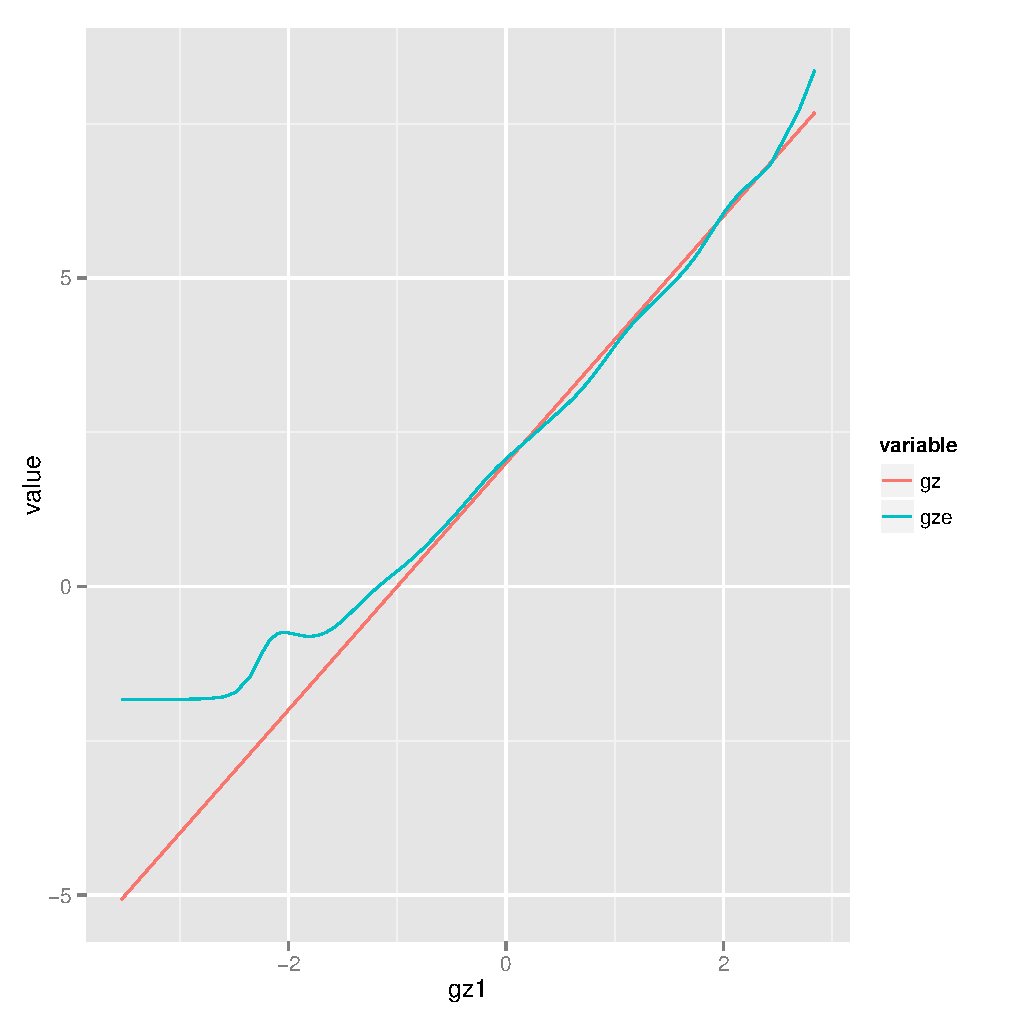
\includegraphics[width=0.9\textwidth]{gzeplot.pdf}
\label{fig:gzplot.pdf}
\end{minipage}
\begin{minipage}[b]{0.5\textwidth}
\centering
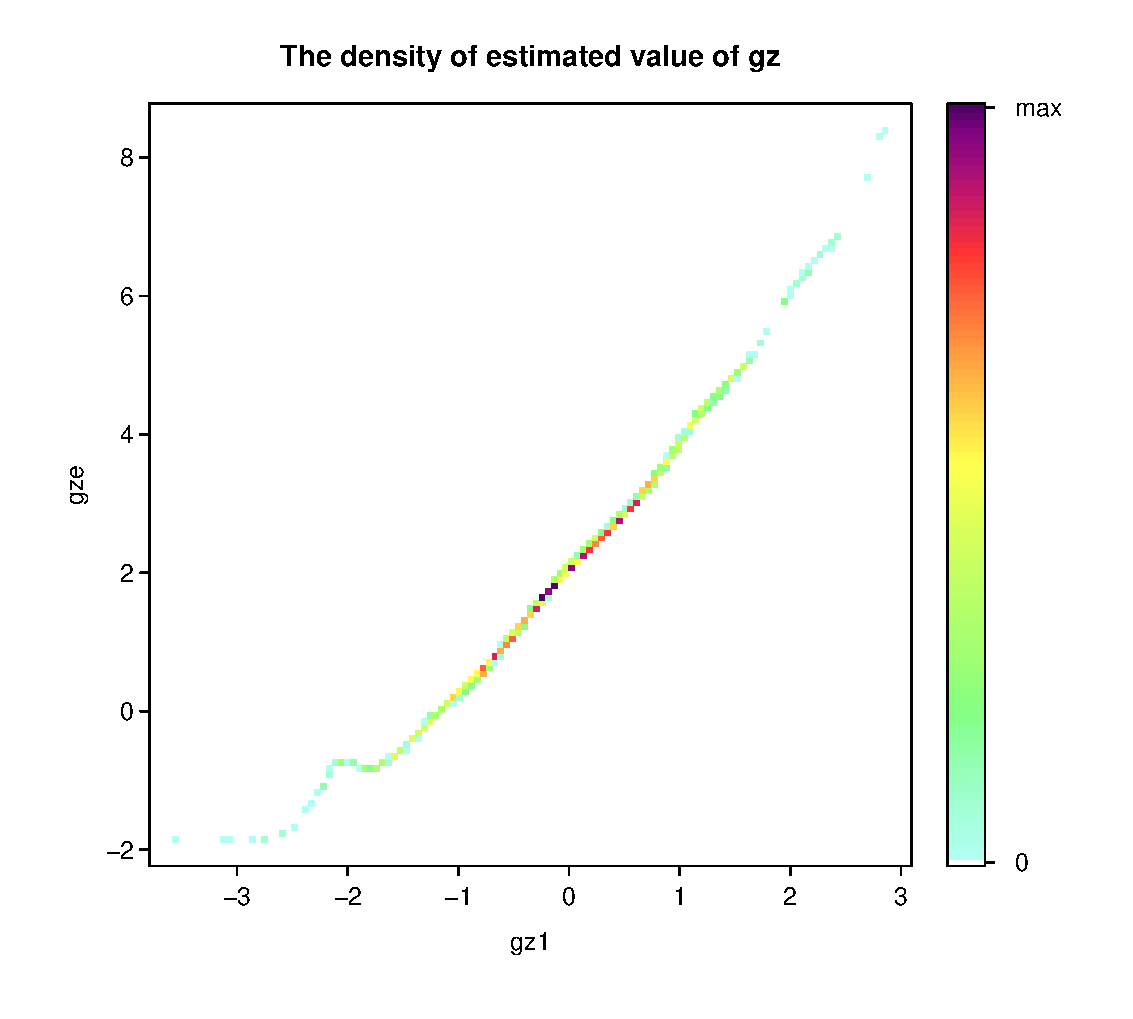
\includegraphics[width=0.9\textwidth]{density.pdf}
\label{fig:density.pdf}
\end{minipage}

\section{Larger sample size?}
Consider a larger sample size ($=10000$), since it may takes few days to run the program, we have bootstraps method to calculate the optimal bandwidth $h$, in our sample selection, we randomly choose 100 from the population 10000 for 100 times. Every time $k$, we compute the constant $c_{1k}$ and $c_{2k}$ such that
\begin{equation}
h^{\text{opt}}_{k} = (c_{1k} Z^{\text{sd}}_{1k}n^{-1/6} , c_{2k} Z^{\text{sd}}_{2k}n^{-1/6})
\end{equation}
where $n=100$ is the sample size we randomly chosen, $k(=1,\ldots,100)$ is the seclection index. $h^{opt}_{k}$ is the optimal bandwidth when considering the LSCV in our subsample $k$ whose size is 100.

Once we get $c_{k}=(c_{1k},c_{2k})$ (the data is stored in ``hs.csv''), we use the mean of the $c_{k}$ ($\bar{c}=(0.8448261, 0.8648953)$) to compute the optimal bandwidth of the full sample ($h=(0.1799968, 0.1845503)$). Given the optimal bandwidth $h$, we can get $\beta = (b_{1},b_{2})$ estimated. With Robinson\rq{}s method and Density Weighted method, we have results presented in table \ref{tab:fullsample10000}. As the table indicates, the standard error of $\beta$ reduces as the sample size increasing from 1000 to 10000, the estimates converges to 1 more accurately.
\begin{table}[htbp]
  \centering
  \caption{Estimation of $\beta$ when sample size is 10000}
    \begin{tabular}{cccc}
    \toprule
    estimates & method & Robinson Method & Density Weighted Method \\
    \midrule
    \multirow{2}[1]{*}{$b_{1}$} & 1     & 1.0063 & 0.97582 \\
          & -     & (0.02568) & (0.01846) \\
    \multirow{2}[1]{*}{$b_{2}$} & 1     & 1.00761 & 0.99749 \\
          & -     & (0.02555) & (0.01831) \\
    \bottomrule
    \end{tabular}%
  \label{tab:fullsample10000}%
\end{table}%
We can use ``cgz'' function to compute $\hat{g}(z_{1},z_{2}|z_{1}=0.5,z_{2}=1.2)=3.145081$. As the previous part shows, we can get the estimated nonparametric component, the following figure shows the estimated curve $\hat{g}(z_{1},z_{2}|z_{2}=1)$. It turns out to be more accurate as the sample size becomes 10000.

\begin{minipage}[b]{0.5\textwidth}
\centering
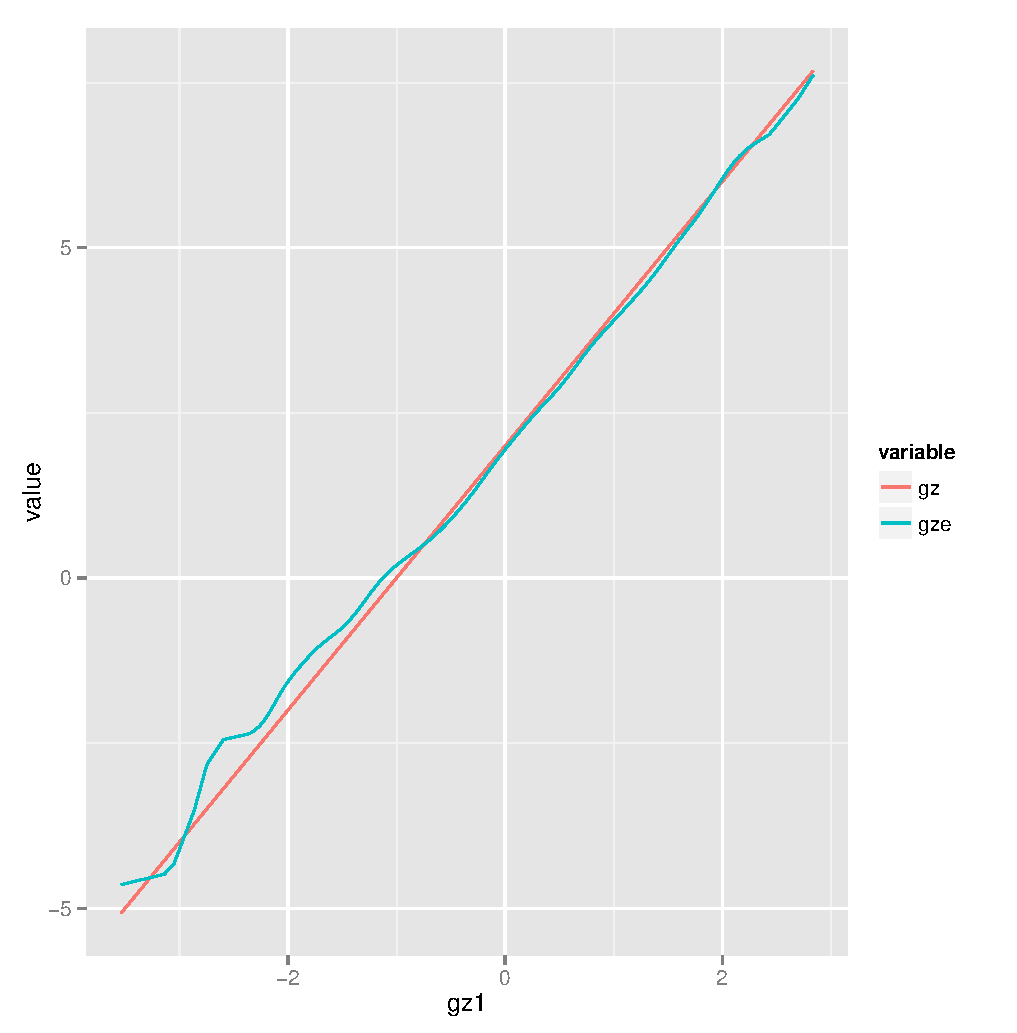
\includegraphics[width=0.9\textwidth]{gzeplot2.pdf}
\label{fig:gzplot2.pdf}
\end{minipage}
\begin{minipage}[b]{0.5\textwidth}
\centering
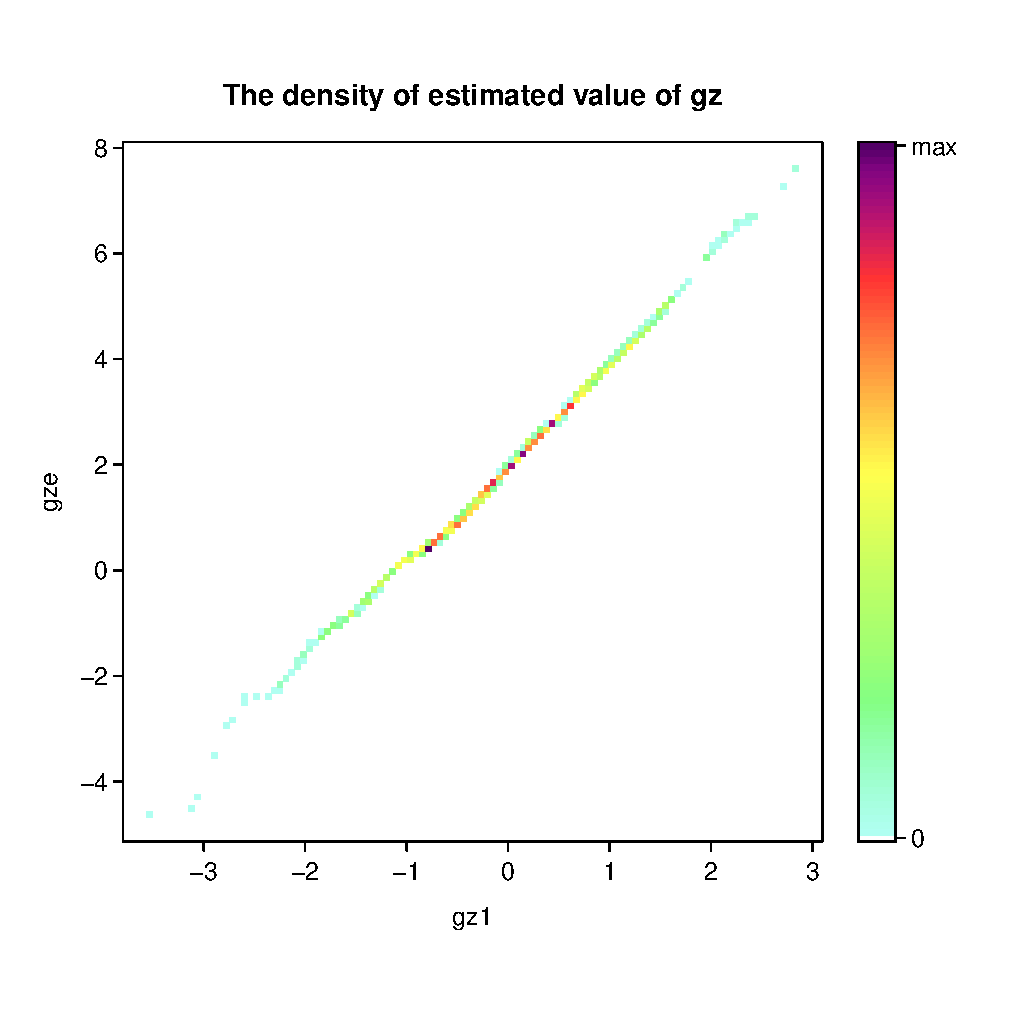
\includegraphics[width=0.9\textwidth]{density2.pdf}
\label{fig:density2.pdf}
\end{minipage}

\section{Semiparametric Partially Linear Model Theory}
\subsection{Estimation of Parametric Linear Component}
A semiparametric partially linear model is given by
\begin{equation}
Y_{i} = X_{i}^{\prime}\beta + g(Z_{i}) + u_{i},\quad i = 1,\ldots,n,
\end{equation}

We have feasible estimation of $\beta$ given by
\begin{equation}
\hat{\beta} = \Big[\sum_{i=1}^{n}\tilde{X}_{i}\tilde{X}_{i}^{\prime}\Big]^{-1}\sum_{i=1}^{n}\tilde{X}_{i}\tilde{Y}_{i}.
\end{equation}
where $\tilde{X}_{i}=X_{i}-\hat{X}_{i}$, and $\tilde{Y}_{i}=Y_{i}-\hat{Y}_{i}$, and
\begin{align}
\hat{Y}_{i} &\equiv \hat{\mathbf{E}}(Y_{i}| Z_{i})\defeq\frac{1}{n}\sum_{j=1}^{n}Y_{j}K_{h}(Z_{i},Z_{j})/\hat{f}(Z_{i})\\
\hat{X}_{i} &\equiv \hat{\mathbf{E}}(X_{i}| Z_{i})\defeq\frac{1}{n}\sum_{j=1}^{n}X_{j}K_{h}(Z_{i},Z_{j})/\hat{f}(Z_{i})
\end{align}
and
\begin{equation}
\hat{f}(Z_{i}) = \frac{1}{n}\sum_{j=1}^{n} K_{h}(Z_{i},Z_{j})
\end{equation}
where
\begin{equation}
K_{h}(Z_{i},Z_{j}) = \prod_{s=1}^{q} \frac{1}{h_{s}}k(\frac{Z_{is}-Z_{js}}{h_{s}}). \label{Kh}
\end{equation}

With Density--Weighted method (By Li 1996), we have
\begin{equation}
    f(Z_{i})\tilde{Y}_{i}  = \big(f(Z_{i})\tilde{X}_{i}\big)^{\prime}\beta + f(Z_{i})u_{i}
\end{equation}
then use OLS to estimate $\beta$.

\subsection{Estimation of the Nonparametric Component}
We know $g(Z_{i})=\mathbf{E}(Y_{i}-X_{i}^{\prime}\beta|Z_{i})$. Therefore, after obtaining a $\sqrt{n}-$ consistent estimator of $\beta$, a consistent estimator of $g(z)$ is given by
\begin{equation}
\hat{g}(z) = \frac{\sum_{j=1}^{n}(Y_{i}-X_{j}^{\prime}\hat{\beta})K_{h}(z,Z_{j})}{\sum_{j=1}^{n}K_{h}(z,Z_{j})}. \label{nonparametric component}
\end{equation}

\subsection{Optimal bandwidth using LSCV}
All the previous theory part is based on the key variable $h$, we can use the $h$ which the \textbf{Rule of Thumb} indicates, i.e.
\begin{equation}
 h \approx 1.06\sigma n^{-1/(q+4)} \approx 1.06 X_{sd}n^{-1/(q+4)}
 \end{equation}
More precisely, we use least squares cross-validation (LSCV) to choose $h_{1},\ldots,h_{q}$. That is, one can always choose $h_{1},\ldots,h_{q}$ to minimize
\begin{equation}
\sum_{i=1}^{n}\Big[Y_{i}-X^{\prime}_{i}\hat{\beta}-g_{-i}(Z_{i},h)\Big]^{2} \label{lscv}
\end{equation}
where
\begin{equation}
\hat{g}_{-i}(Z_{i},h) = \frac{\sum_{j\not=i}(Y_{j}-X_{j}^{\prime}\hat{\beta})K_{h}(Z_{i},Z_{j})}{\sum_{j\not=i}K_{h}(Z_{i},Z_{j})}
\end{equation}

We can choose $h$ and estimate $\beta$ simultaneously since once we get $h$, we can get the estimates of $\beta$.
\subsection{Kernel Function}
We can use different kernel functions to estimate the pdf.

A uniform kernel function is given by
\begin{equation}\label{uniform ker}
k(z)=
\begin{cases}
1/2 & \text{if\,} |z|\leq 1 \\
0   & \text{otherwise,}
\end{cases}
\end{equation}

A standard normal kernel is given by
\begin{equation}
    k(v) = \frac{1}{\sqrt{\,2\pi}}e^{-\frac{1}{2}v^{2}}\label{std normal ker}
\end{equation}

In my code, one can choose either way to use. By default, I use standard normal kernel, if you want to use uniform kernel, just comment the line 16 in \textit{semi.R}, and uncomment the line 17.
\end{document}
